\documentclass{standalone}
%
\usepackage{tikz}
\usetikzlibrary{backgrounds,arrows.meta,shapes.callouts}
\usepackage{xcolor}
%
\definecolor{space}{HTML}{1F2C4E}
\definecolor{earth}{HTML}{0089FA}
\definecolor{dida}{HTML}{FFDE00}
\definecolor{title}{HTML}{FBA706}
%
\usepackage{fontspec}
\setmainfont{Open Dyslexic}
%
\title{Vita di un asteroide}
\begin{document}
	\tikzset{
		partial ellipse/.style args = {#1:#2:#3}{insert path={+ (#1:#3) arc (#1:#2:#3)}},
		notice/.style  = { draw, ellipse callout, callout relative pointer={#1} },
	}
	\begin{tikzpicture}[background rectangle/.style={fill=white},show background rectangle,>={[inset=0,angle'=27]Stealth}]
		%title
		\draw [black,ultra thick,fill=title] (0,9.8) rectangle (30,13.3);
		\node at (15,11.8) {\textcolor{black}{\fontsize{75}{76}\selectfont Vita di un asteroide}};
		%
		\begin{scope}[shift={(0,1.5)}]
			\draw [ultra thick, fill=space] (1,0) rectangle (29,-2);
		\end{scope}
		%
		\begin{scope}[shift={(0,5)}]
			\draw [ultra thick, fill=earth] (20.5,4) rectangle (25.5,-4);
			\node at (23,0) {
\includegraphics[width=5cm]{carl_sagan}};
			\node (example-textwidth-2) [notice={(3,0.5)}, ultra thick, right, align=center, text width=12cm, color=black, fill=white, font=\fontsize{23pt}{24pt}\selectfont] at (1,-1) {La fascia principale degli asteroidi è una "striscia" compresa tra le orbite di Marte e Giove.};
		\end{scope}
		%
		\begin{scope}[shift={(0,-3)}]
			\draw [ultra thick, fill=earth] (5.5,4) rectangle (10.5,-4);
			\node at (8,0) {
\includegraphics[width=5cm]{carl_sagan}};
			\node (example-textwidth-2) [notice={(-3,0.5)}, ultra thick, right, align=center, text width=12cm, color=black, fill=white, font=\fontsize{23pt}{24pt}\selectfont] at (12,-1) {Vi si trovano alcune migliaia di rocce spaziali dette... \textbf{asteroidi}!};
		\end{scope}
		% Fascia asteroidi
		\begin{scope}[shift={(0,-13)}]
			\draw [fill=space, ultra thick] (1,5) rectangle (28,-5);
			\node at (15,0) {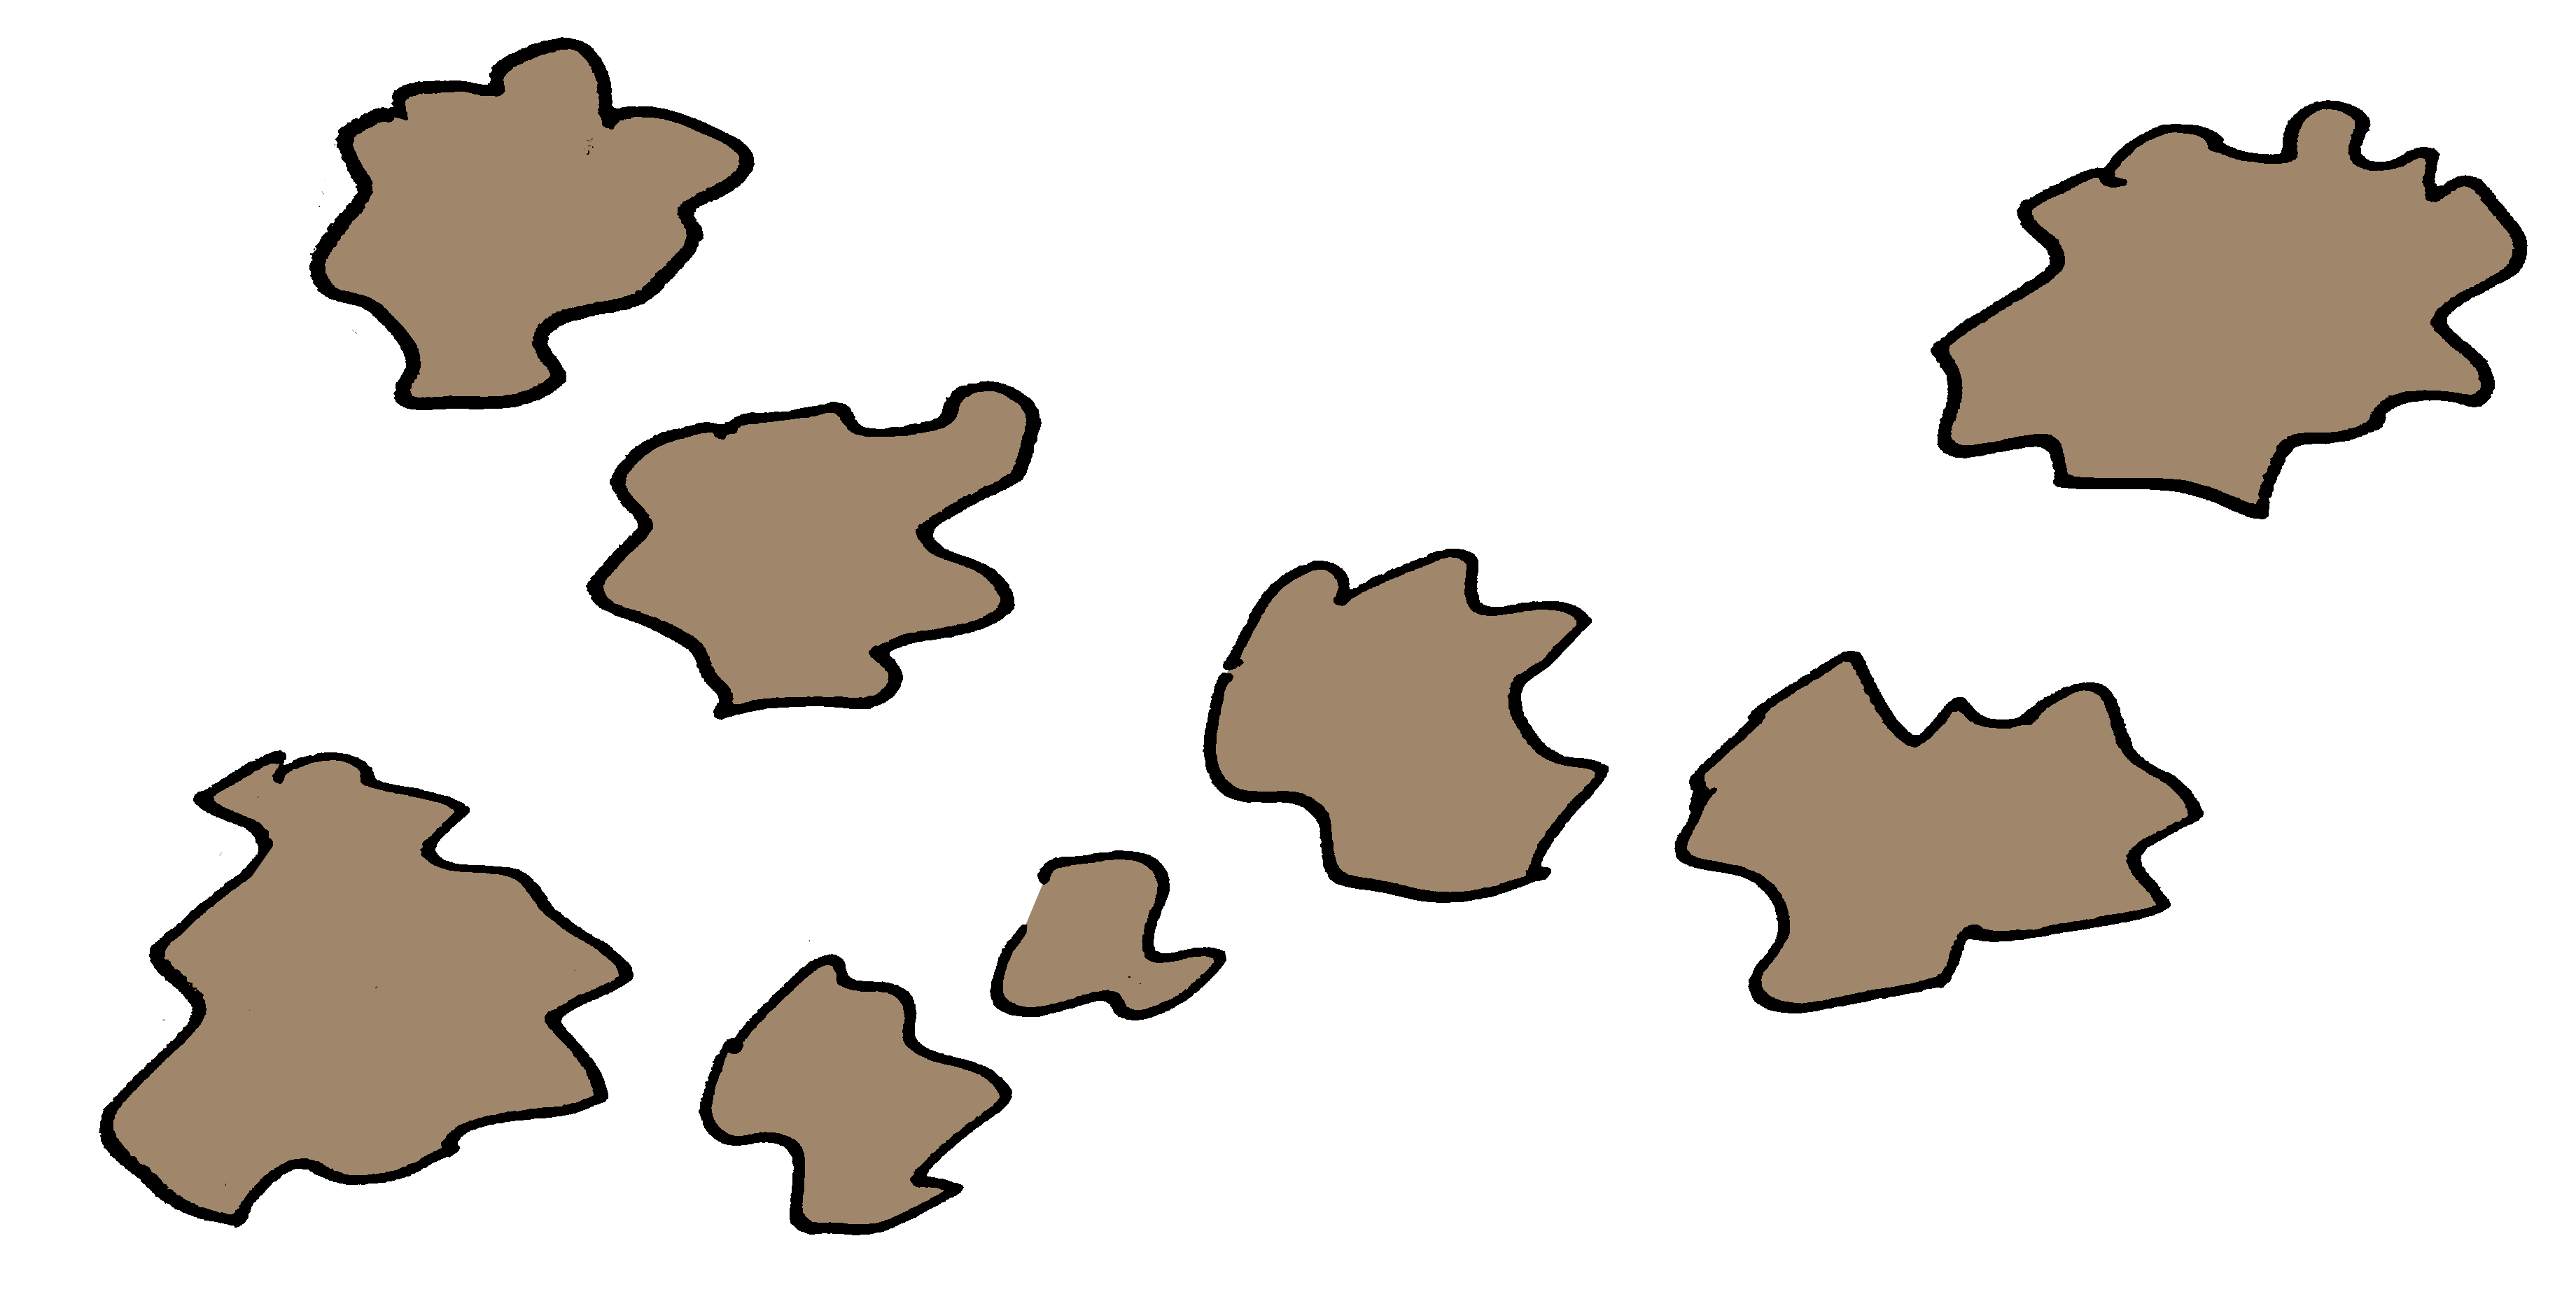
\includegraphics[width=20cm]{fascia_asteroidi}};
		\end{scope}
		% Collisione
		\begin{scope}[shift={(0,-21.5)}]
			\draw [fill=dida, ultra thick] (2,4) rectangle (27.5,1);
			%
			\node (example-textwidth-2) [right, align=left, text width=25cm, color=black, font=\fontsize{23pt}{24pt}\selectfont] at (2.5,2.5) {Ogni tanto qualcuna di queste rocce viene catturata dall'attrazione gravitazionale di un altro corpo celeste, magari a causa di una collisione improvvisa...};
			\node at (8,-3) {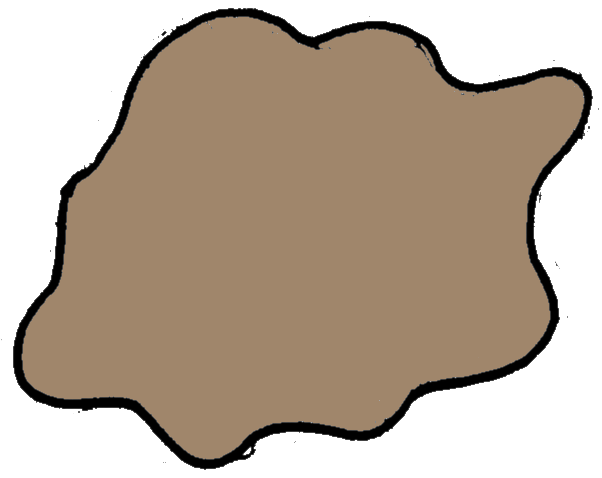
\includegraphics[width=5cm]{asteroide01}};
			\node at (14,-2) {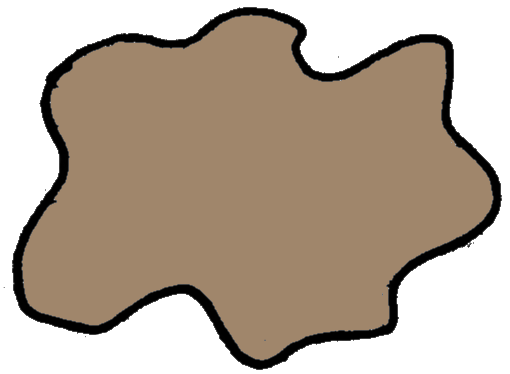
\includegraphics[width=5cm]{asteroide02}};
			%
			\node at (22,-9) {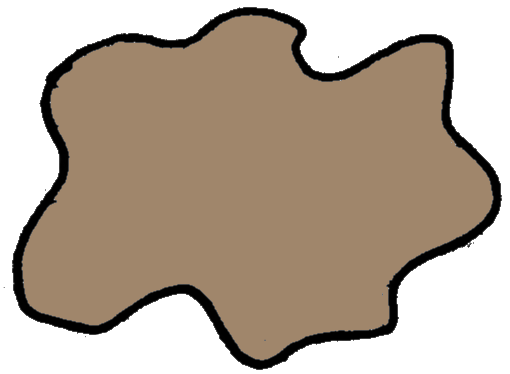
\includegraphics[width=5cm]{asteroide02}};
			\node at (20.5,-9) {
\includegraphics[width=4cm]{sbonk}};
			\node at (18,-10) {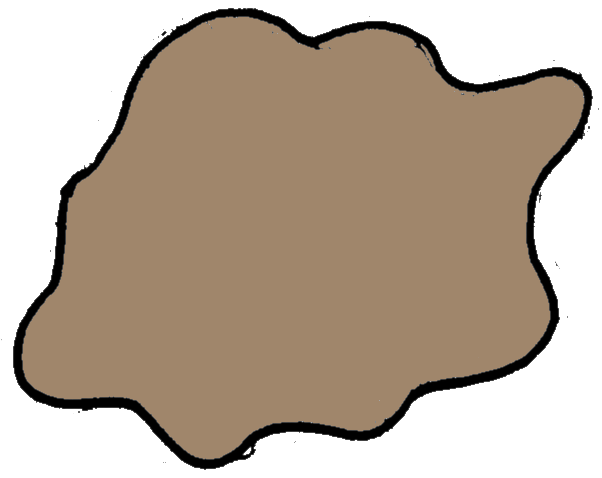
\includegraphics[width=5cm]{asteroide01}};
			%
			\node at (23,-16) {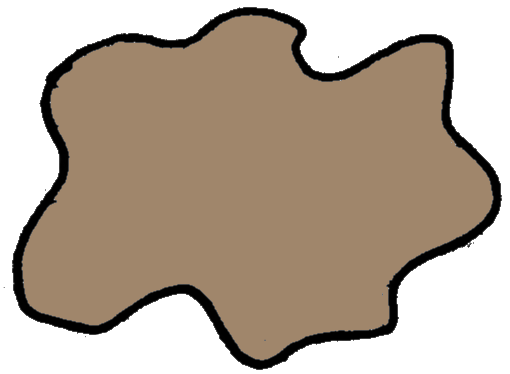
\includegraphics[width=5cm]{asteroide02}};
			\node at (4,-19) {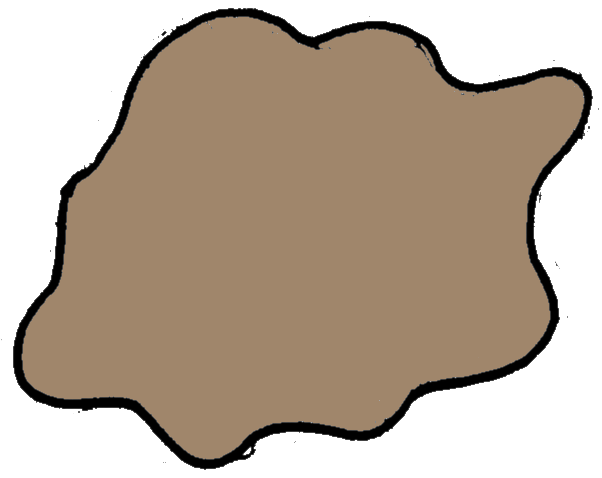
\includegraphics[width=5cm]{asteroide01}};
			%
			\node (example-textwidth-2) [notice={(-2,-0.5)}, ultra thick, right, align=center, text width=6cm, color=black, fill=white, font=\fontsize{23pt}{24pt}\selectfont] at (7,-16) {Ma chi ti ha dato la patente!};
			\node (example-textwidth-2) [notice={(2,0.5)}, ultra thick, right, align=center, text width=4cm, color=black, fill=white, font=\fontsize{23pt}{24pt}\selectfont] at (13,-19) {Isaac Newton!};
		\end{scope}
		% urto con la Terra
		\begin{scope}[shift={(0,-48)}]
			\draw [fill=space, ultra thick] (1.5,3) rectangle (28,-36);
			\draw [fill=dida, ultra thick] (2,4) rectangle (27.5,0.8);
			\node (example-textwidth-2) [right, align=left, text width=25cm, color=black, font=\fontsize{23pt}{24pt}\selectfont] at (2.5,2.5) {Il cambio di traiettoria potrebbe portare l'asteroide in rotta di collisiane con altri pianeti. Come la Terra...};
			\node at (23,-2) {
\includegraphics[width=5cm]{asteroide03}};
			\node at (5,-4) {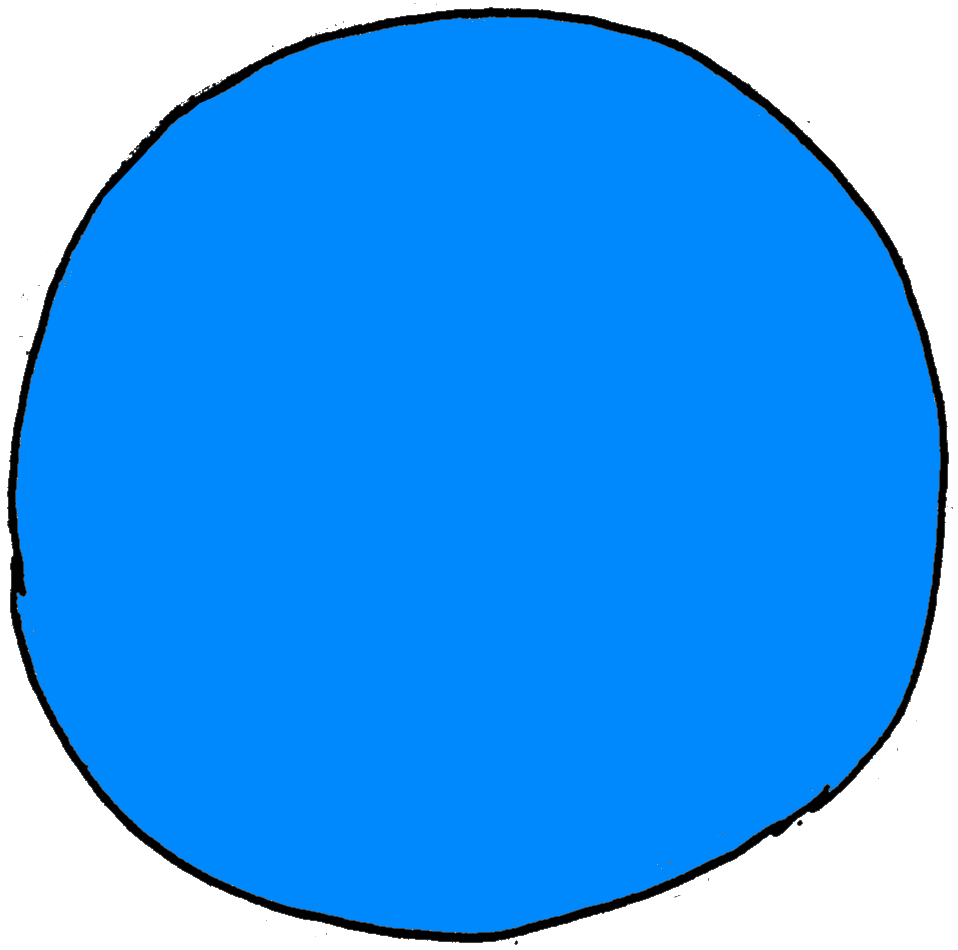
\includegraphics[width=3cm]{terra}};
			\node (example-textwidth-2) [notice={(2,0.5)}, ultra thick, right, align=center, text width=8cm, color=black, fill=white, font=\fontsize{23pt}{24pt}\selectfont] at (9,-5) {Oh no! Sto andando verso la Terra! Lì non si trova mai un parcheggio!};
			\node at (15,-14) {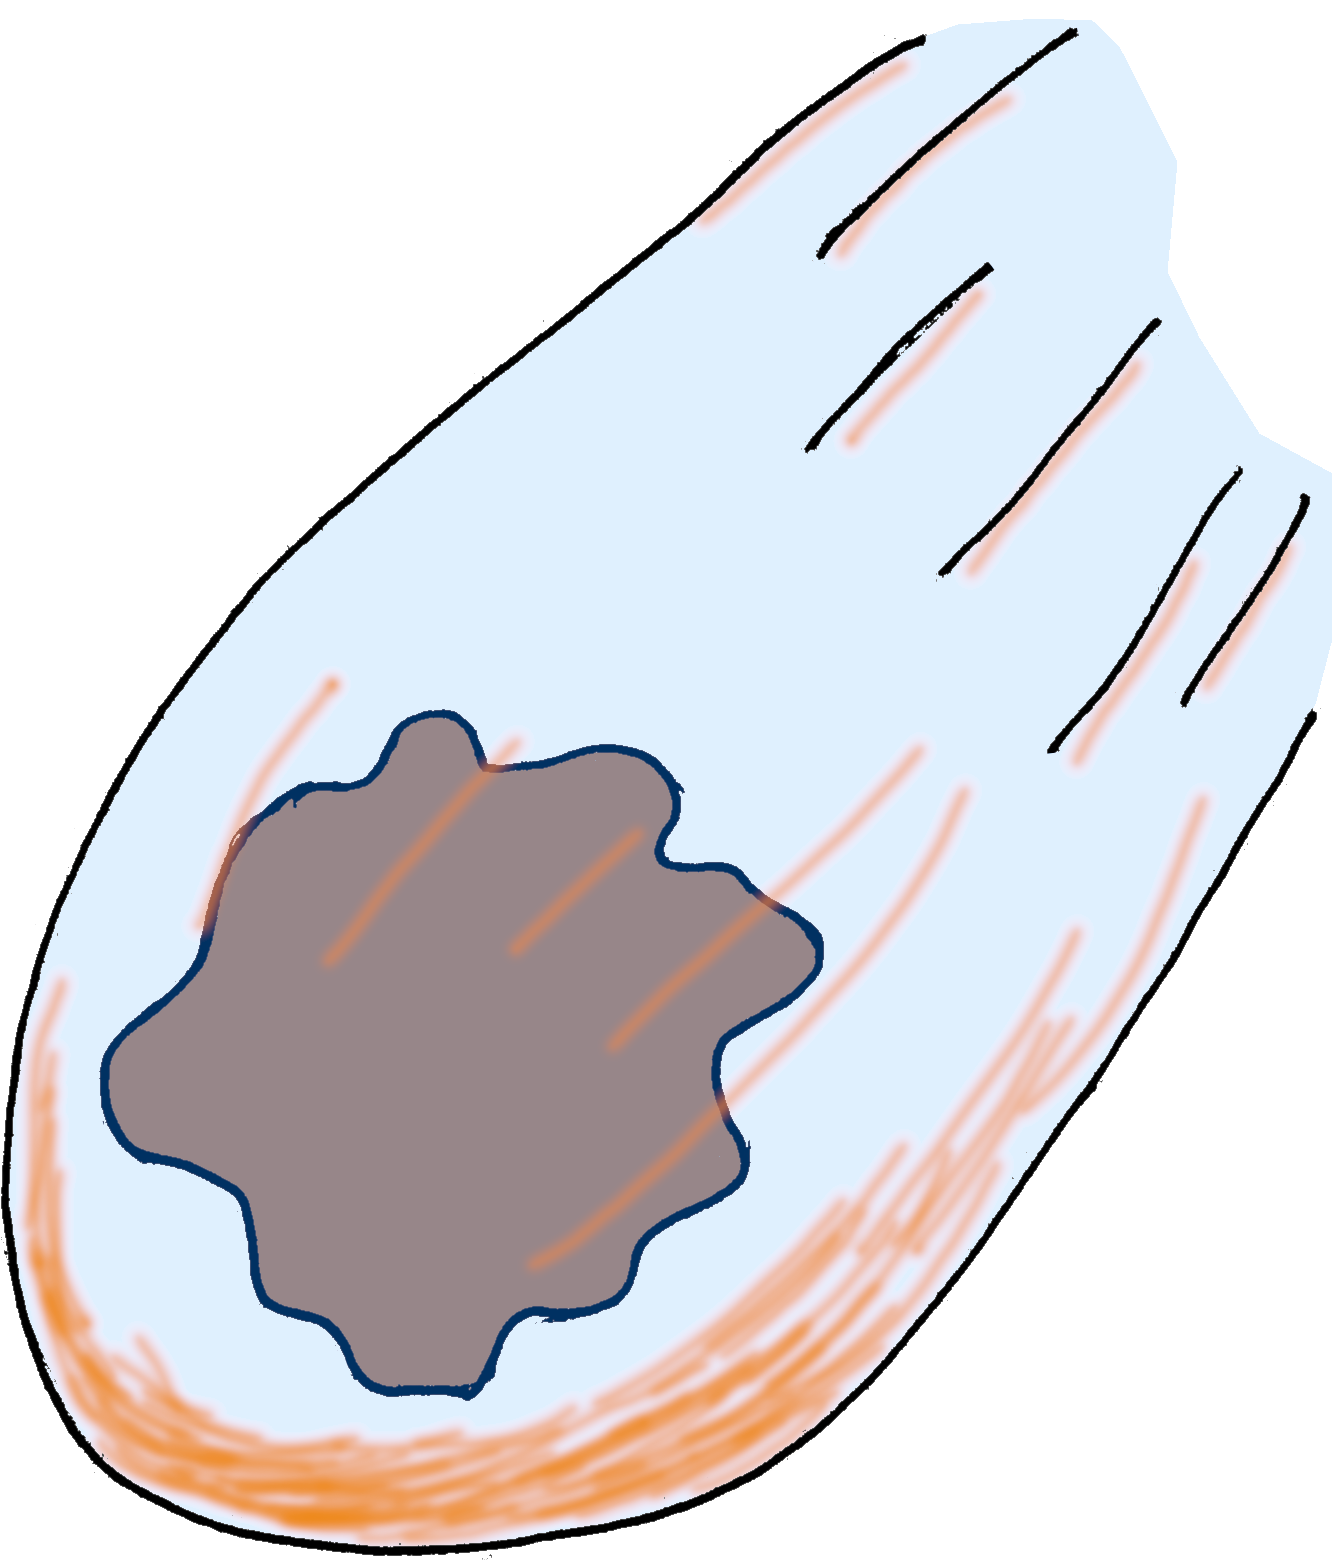
\includegraphics[width=8cm]{asteroide_in}};
			\node (example-textwidth-2) [notice={(2,0.5)}, ultra thick, right, align=center, text width=6cm, color=black, fill=white, font=\fontsize{23pt}{24pt}\selectfont] at (2,-18) {Inizia a fare un po' caldo...};
			\node at (7,-26) {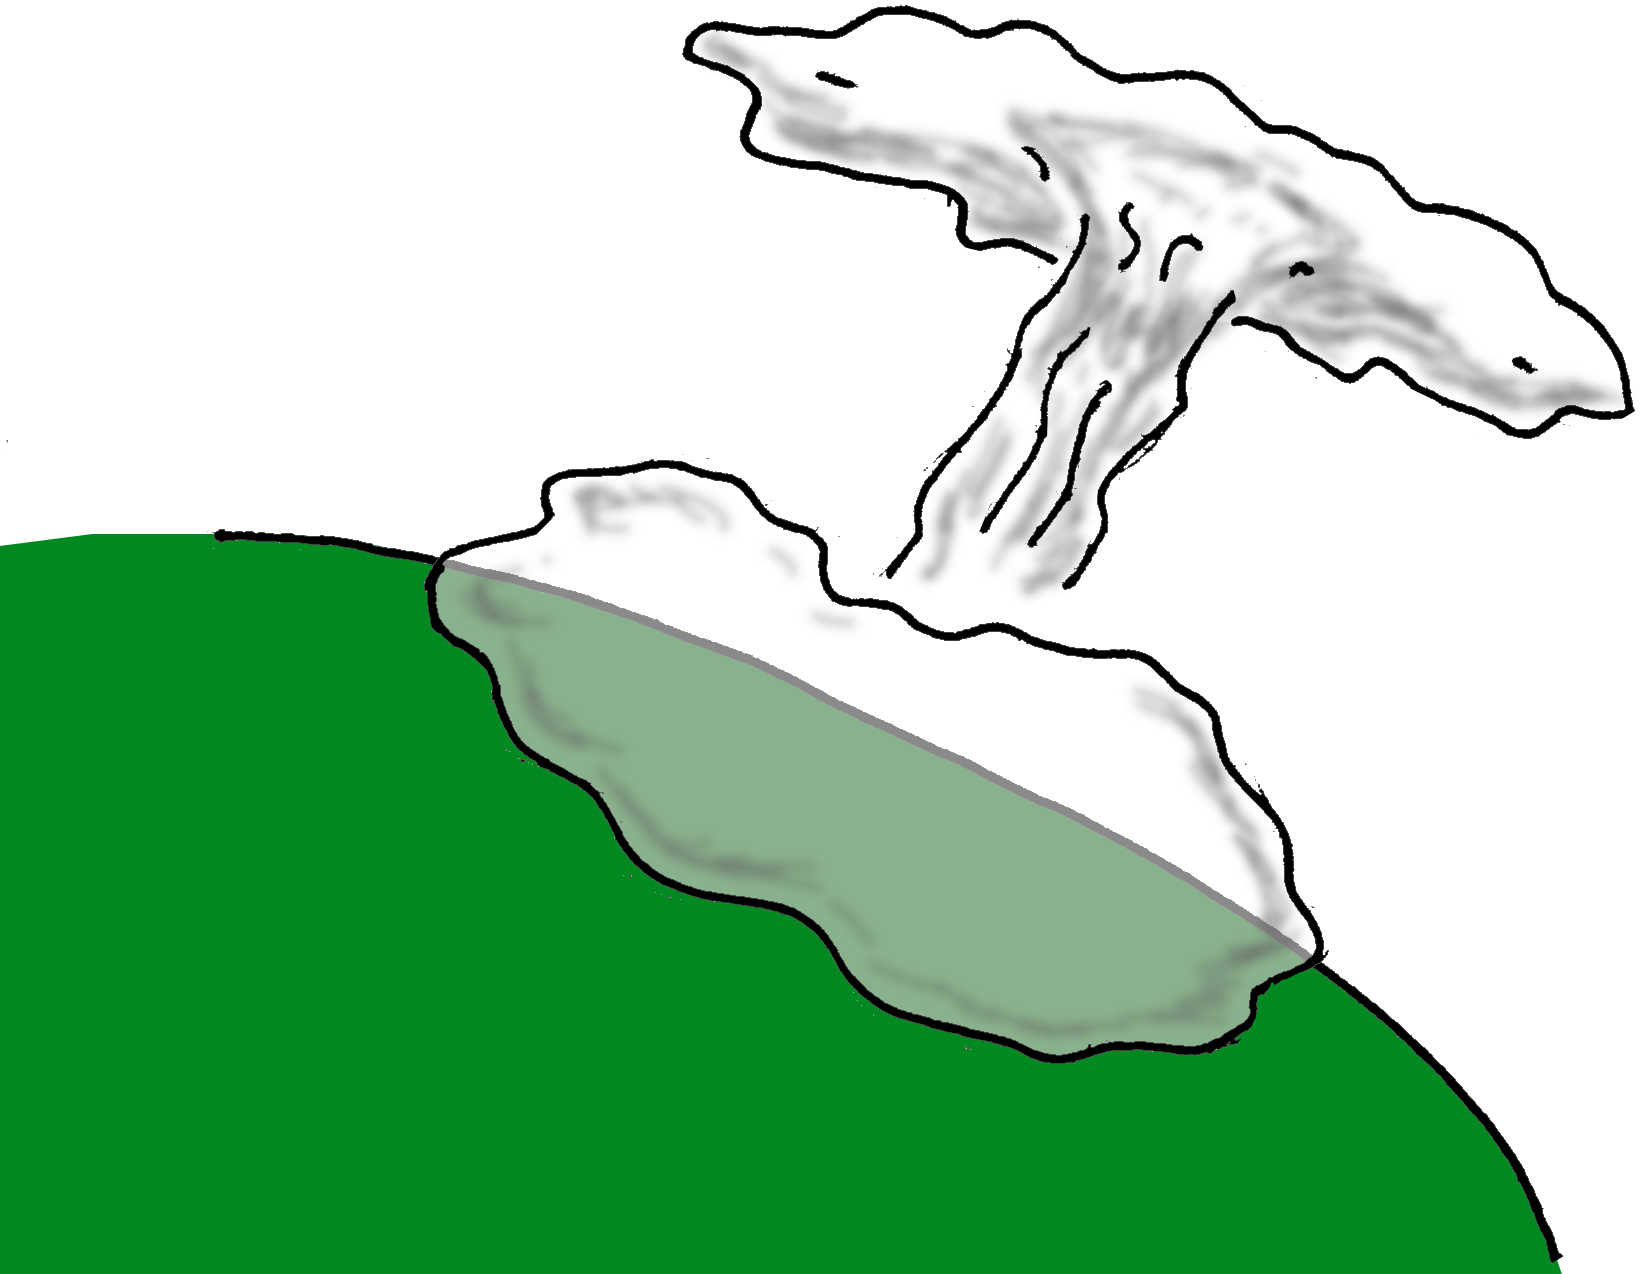
\includegraphics[width=12cm]{urto}};
			\node at (22.5,-30) {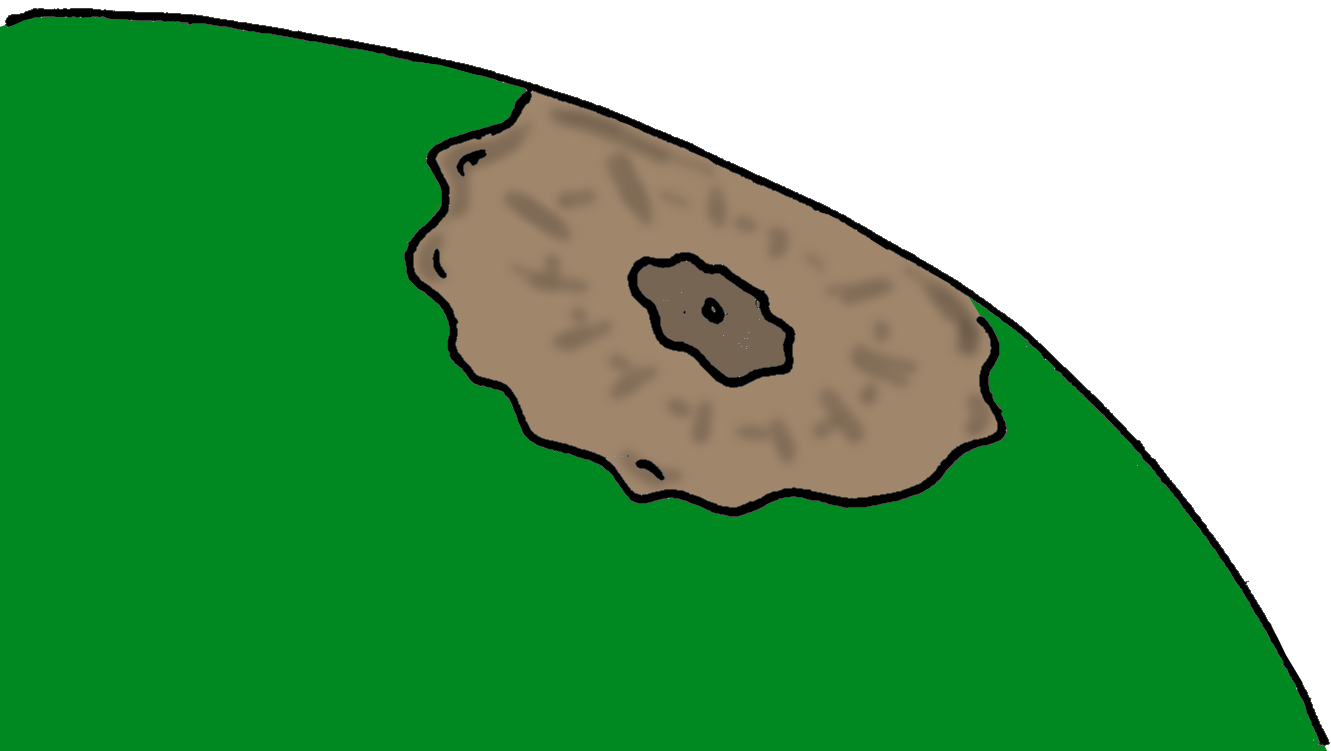
\includegraphics[width=12cm]{cratere}};
			\node (example-textwidth-2) [notice={(-2,-0.5)}, ultra thick, right, align=center, text width=10cm, color=black, fill=white, font=\fontsize{23pt}{24pt}\selectfont] at (12,-25) {Che botta! Mi serve un momento per riprendermi...};
		\end{scope}
		%
		\begin{scope}[shift={(0,-83)}]
			\draw [ultra thick, fill=earth] (5.5,4) rectangle (10.5,-4);
			\node at (8,0) {
\includegraphics[width=5cm]{carl_sagan}};
			\node (example-textwidth-2) [notice={(-3,0.5)}, ultra thick, right, align=center, text width=12cm, color=black, fill=white, font=\fontsize{23pt}{24pt}\selectfont] at (12,-1) {E del nostro amico asteroide restò solo un cratere...};
		\end{scope}
		% Moriarty
		\begin{scope}[shift={(0,-92)}]
			\draw [fill=dida, ultra thick] (2,4.5) rectangle (27.5,0.5);
			\node (example-textwidth-2) [right, align=left, text width=25cm, color=black, font=\fontsize{23pt}{24pt}\selectfont] at (2.5,2.5) {Secondo la teoria del professor Moriarty, la fascia degli asteroidi è nata dall'urto di un pianeta nano con un suo omologo extrasolare.};
			%
			\node at (23,-5) {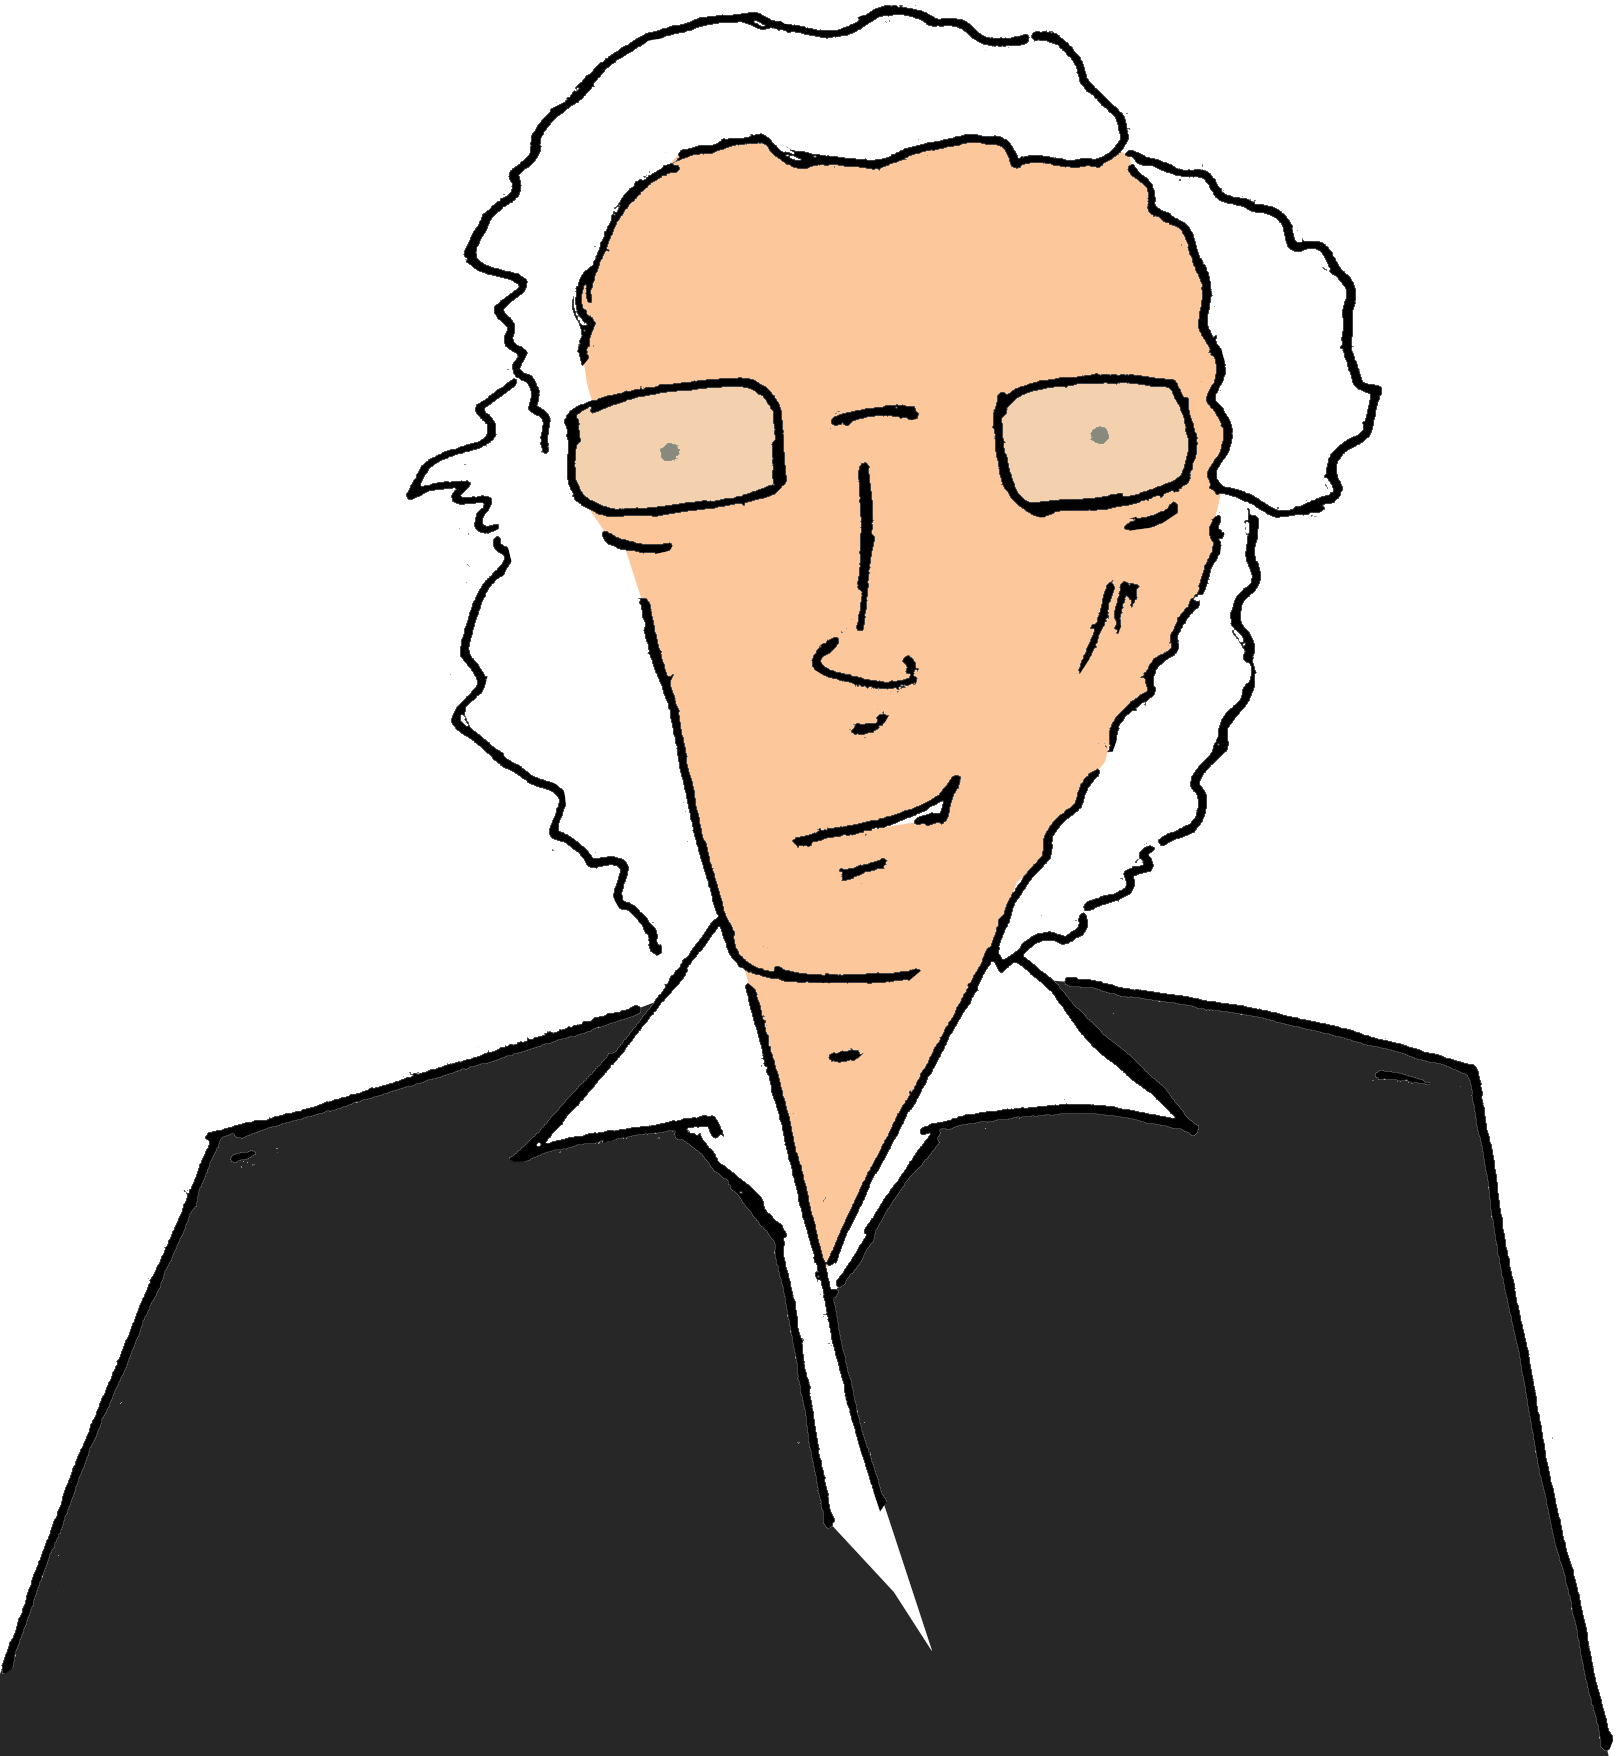
\includegraphics[width=8cm]{asimov}};
			\node (example-textwidth-2) [notice={(3,0.5)}, ultra thick, right, align=center, text width=12cm, color=black, fill=white, font=\fontsize{23pt}{24pt}\selectfont] at (2,-6) {Questa teoria, però, me la sono inventata io per entrare nel club degli \emph{sherlockiani}!};
		\end{scope}
		%
		\begin{scope}[shift={(0,-106)}]
			\node at (8,0) {
\includegraphics[width=5cm]{carl_sagan}};
			\node (example-textwidth-2) [notice={(-3,0.5)}, ultra thick, right, align=center, text width=12cm, color=black, fill=white, font=\fontsize{23pt}{24pt}\selectfont] at (12,-1) {In realtà è stata tutta colpa di Giove che con la sua gravità ha perturbato il moto degli asteroidi impedendo loro di unirsi per formare un pianeta.};
		\end{scope}
		%
		\begin{scope}[shift={(0,-113)}]
			\node at (27,0) () {
\includegraphics[width=3.7cm]{licenza}};
			\node (example-textwidth-2) [right, align=left, text width=14cm, color=black, font=\fontsize{14pt}{15pt}\selectfont] at (11,-0.1) {Testo e illustrazioni (laddove diversamente indicato): @ulaulaman - Gianluigi Filippelli};
		\end{scope}
	\end{tikzpicture}
\end{document}
